
% Age of Aquarius chapter ---------------------------------------------
\chapter*{Age of Aquarius}
\addcontentsline{toc}{chapter}{Age of Aquarius}

\begin{flushright}
\parbox{0.8\textwidth}{
\emph{The greatest difficulty with the world is not its ability to produce, but the unwillingness to share. \\
\hspace*{\fill}{\textperiodcentered \textperiodcentered \textperiodcentered \hspace*{0.2em} Roy L. Smith} } }
\end{flushright}

\noindent
Age of Aquarius is chess variant which is played on 14 x 14 board,
with light yellow and light green fields and light tan-gold and
dark green pieces. In algebraic notation, columns are enumerated
from 'a' to 'n', and rows are enumerated from '1' to '14'. A new
piece is introduced, Unicorn.

\clearpage % ..........................................................

\section*{Unicorn}
\addcontentsline{toc}{section}{Unicorn}

\noindent
\begin{wrapfigure}[5]{l}{0.4\textwidth}
\centering
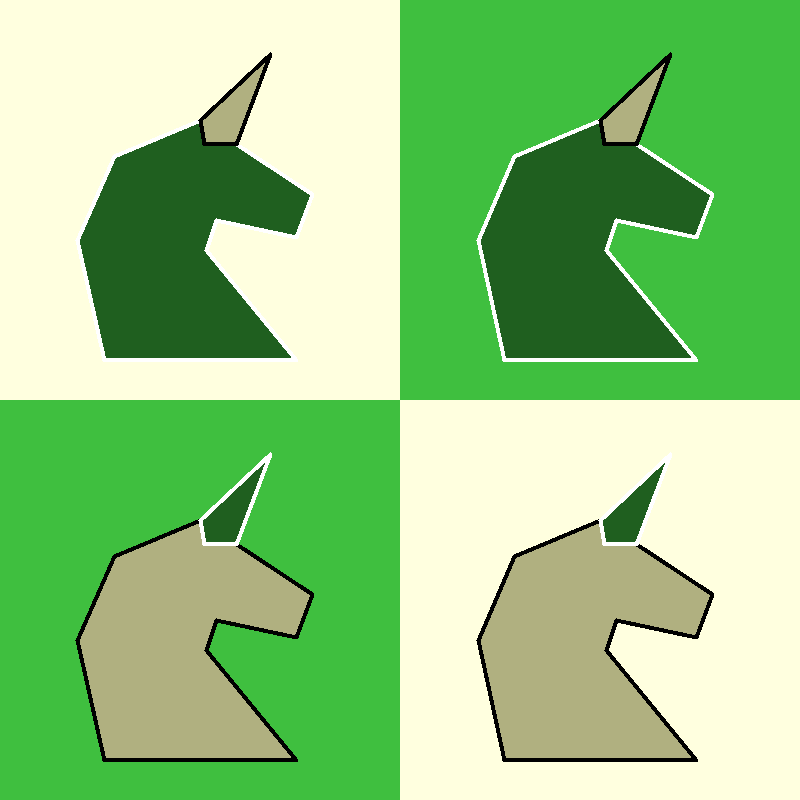
\includegraphics[width=0.4\textwidth, keepaspectratio=true]{pieces/09_unicorn.png}
\caption{Unicorn}
\label{fig:09_unicorn}
\end{wrapfigure}
Unicorn is a piece similar to Knight, only it can jump longer on
opposite color fields. Just as Knight, Unicorn is not obstructed
by any piece in its' surroundings.

\vspace{7\baselineskip}
\subsection*{Movement}
\addcontentsline{toc}{subsection}{Movement}

\noindent
\begin{wrapfigure}{l}{0.4\textwidth}
\centering
\includegraphics[width=0.4\textwidth, keepaspectratio=true]{examples/08_move_unicorn_same_color.png}
\caption{Unicorn short jump}
\label{fig:08_move_unicorn_same_color}
\end{wrapfigure}
On fields with the same color as Unicorn, it can move exactly the
same way Knight does.

\clearpage % ..........................................................

\noindent
\begin{figure}[!h]
% \begin{figure}[!t]
\includegraphics[width=1.0\textwidth, keepaspectratio=true]{examples/08_move_unicorn_opposite_color.png}
\caption{Unicorn long jump}
\label{fig:08_move_unicorn_opposite_color}
% \centering
\end{figure}

On fields in opposite color to Unicorn's, Unicorn can jump much longer.
Again, just as Knight, Unicorn is not hampered by surrouding pieces.
Only own pieces on marked (i.e. step) fields can prevent Unicorn to move.
Opponent's pieces on step-fields would, naturally, be captured.

\clearpage % ..........................................................

\section*{Promotion}
\addcontentsline{toc}{section}{Promotion}

Is not forced...

\textbf{\huge{TODO :: Promotion !!!}} % TODO :: FIX ME !!!

\clearpage % ..........................................................

\section*{En passant}
\addcontentsline{toc}{section}{En passant}

\noindent
\begin{wrapfigure}{l}{0.4\textwidth}
\centering
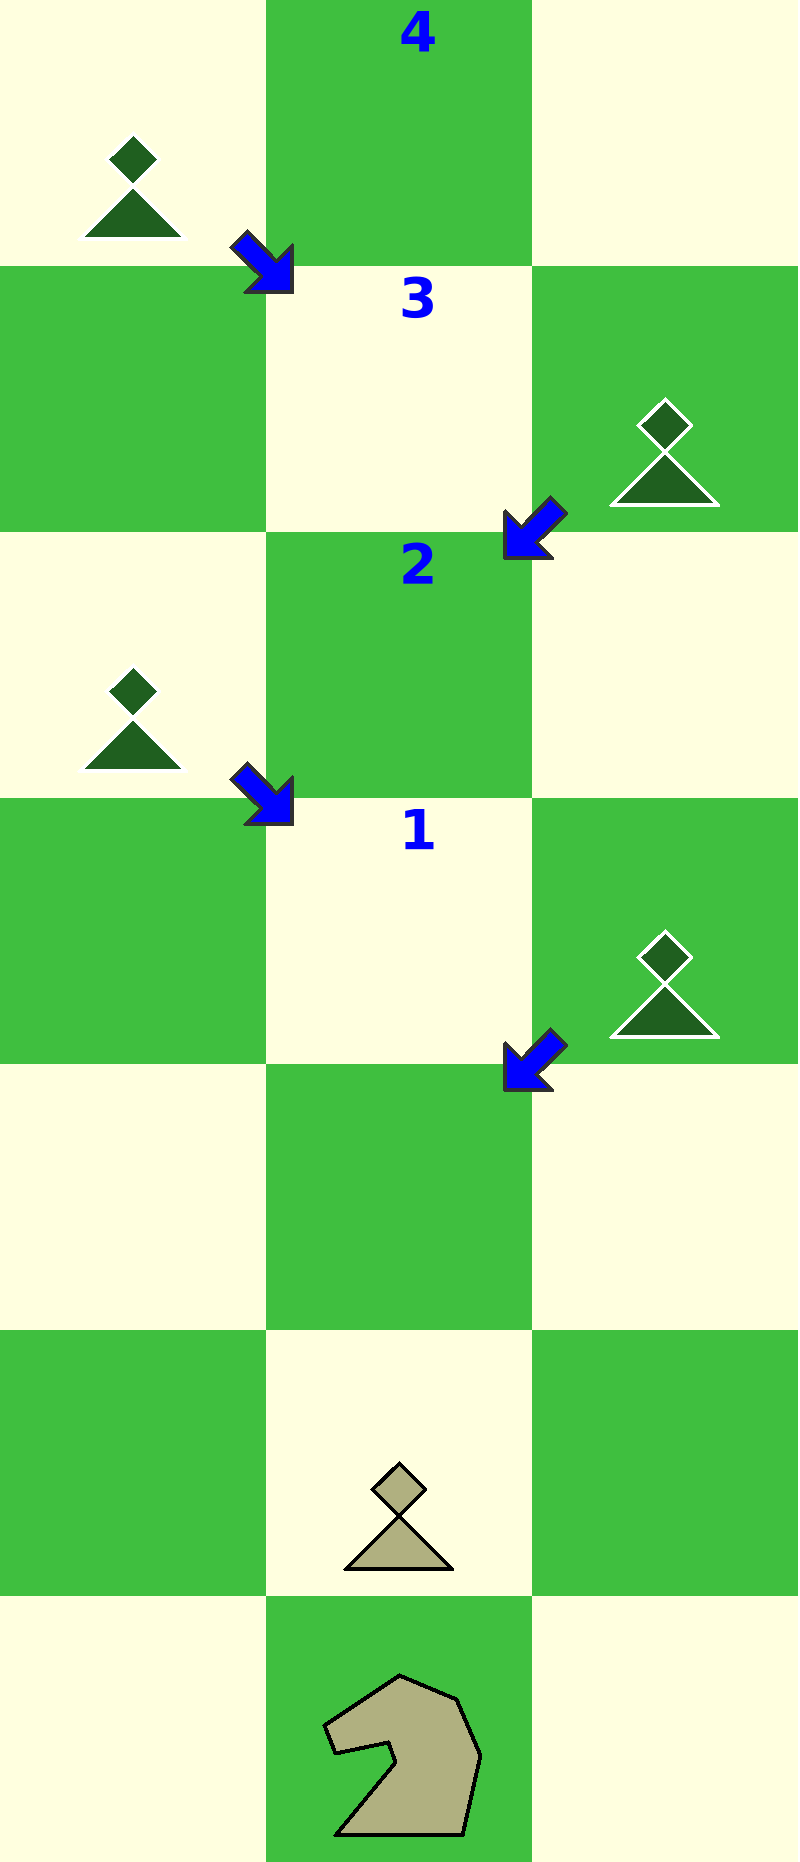
\includegraphics[width=0.214285714286\textwidth, keepaspectratio=true]{en_passants/08_age_of_aquarius_en_passant.png}
\caption{En passant}
\label{fig:08_age_of_aquarius_en_passant}
\end{wrapfigure}
En passant is identical to one in Classic Chess, only difference is that Pawn can now
move longer on initial turn, up to 5 fields in this instance. As expected, all passed-by
opponent's Pawns also gain en passant opportunity.

In example on left, if light Pawn's initial move was 4 fields long, ending in field marked
3, three dark Pawns closest to light Pawn's initial position would have en passant opportunity,
in rows 1, 2 and 3.

\clearpage % ..........................................................

\section*{Castling}
\addcontentsline{toc}{section}{Castling}

Castling is essentially the same as it is in Classical Chess, only real difference is that
King can move 2, 3, 4 or 5 fields across. All other constraints from Classical Chess still
applies.

\noindent
\begin{figure}[!h]
% \begin{figure}[!t]
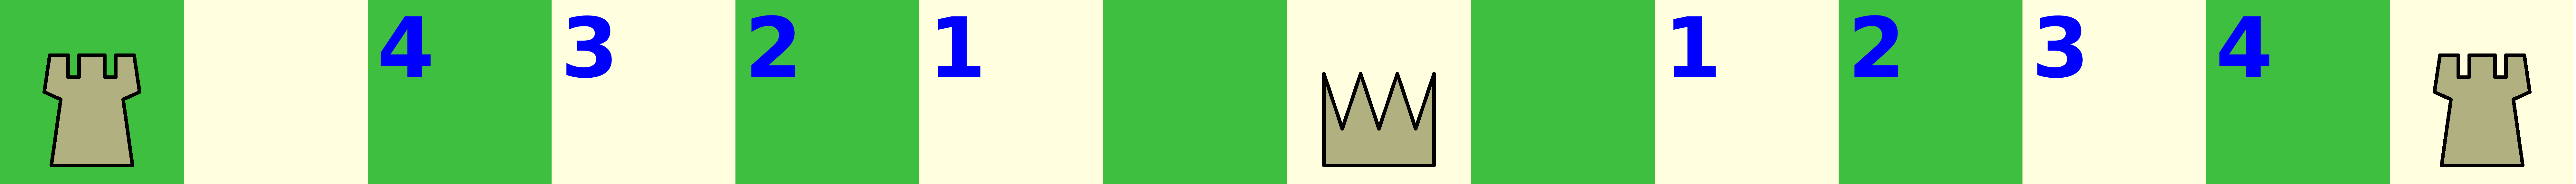
\includegraphics[width=1.0\textwidth, keepaspectratio=true]{castlings/08_age_of_aquarius_castling.png}
\caption{Castling}
\label{fig:08_age_of_aquarius_castling}
% \centering
\end{figure}

In example above, all valid King's castling moves are numbered. Regardless if King performs
long or short castling move, Rook would always end up on the opposite side of King on the
field immediately next to it, i.e. closer to center.

\noindent
\begin{figure}[!h]
% \begin{figure}[!t]
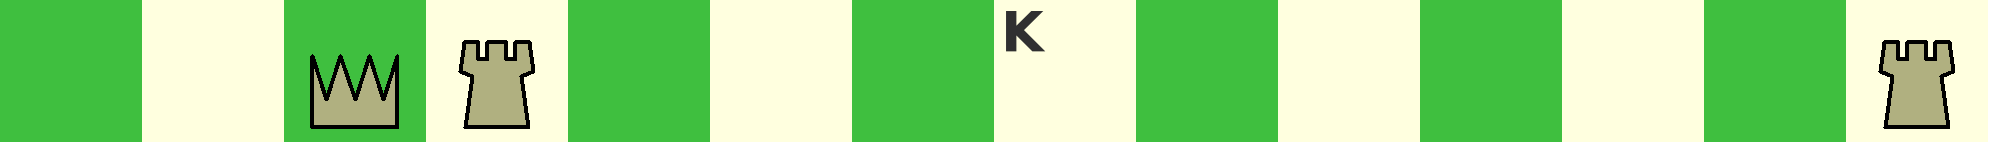
\includegraphics[width=1.0\textwidth, keepaspectratio=true]{castlings/long_left/08_age_of_aquarius_castling_long_left.png}
\caption{Castling long left}
\label{fig:08_age_of_aquarius_castling_long_left}
% \centering
\end{figure}

In this example King was castling long to the left. Initial King's position is marked with "K".
After castling is finished, left Rook ends up at field immediately on the right to the King.

\clearpage % ..........................................................

\section*{Initial setup}
\addcontentsline{toc}{section}{Initial setup}

Compared to initial setup of Mayan Ascendancy, Unicorn is inserted between Pyramid and Knight
symmetrically, on both sides of chessboard. This can be seen in the image below:

\noindent
% \begin{figure}[t]
\begin{figure}[h]
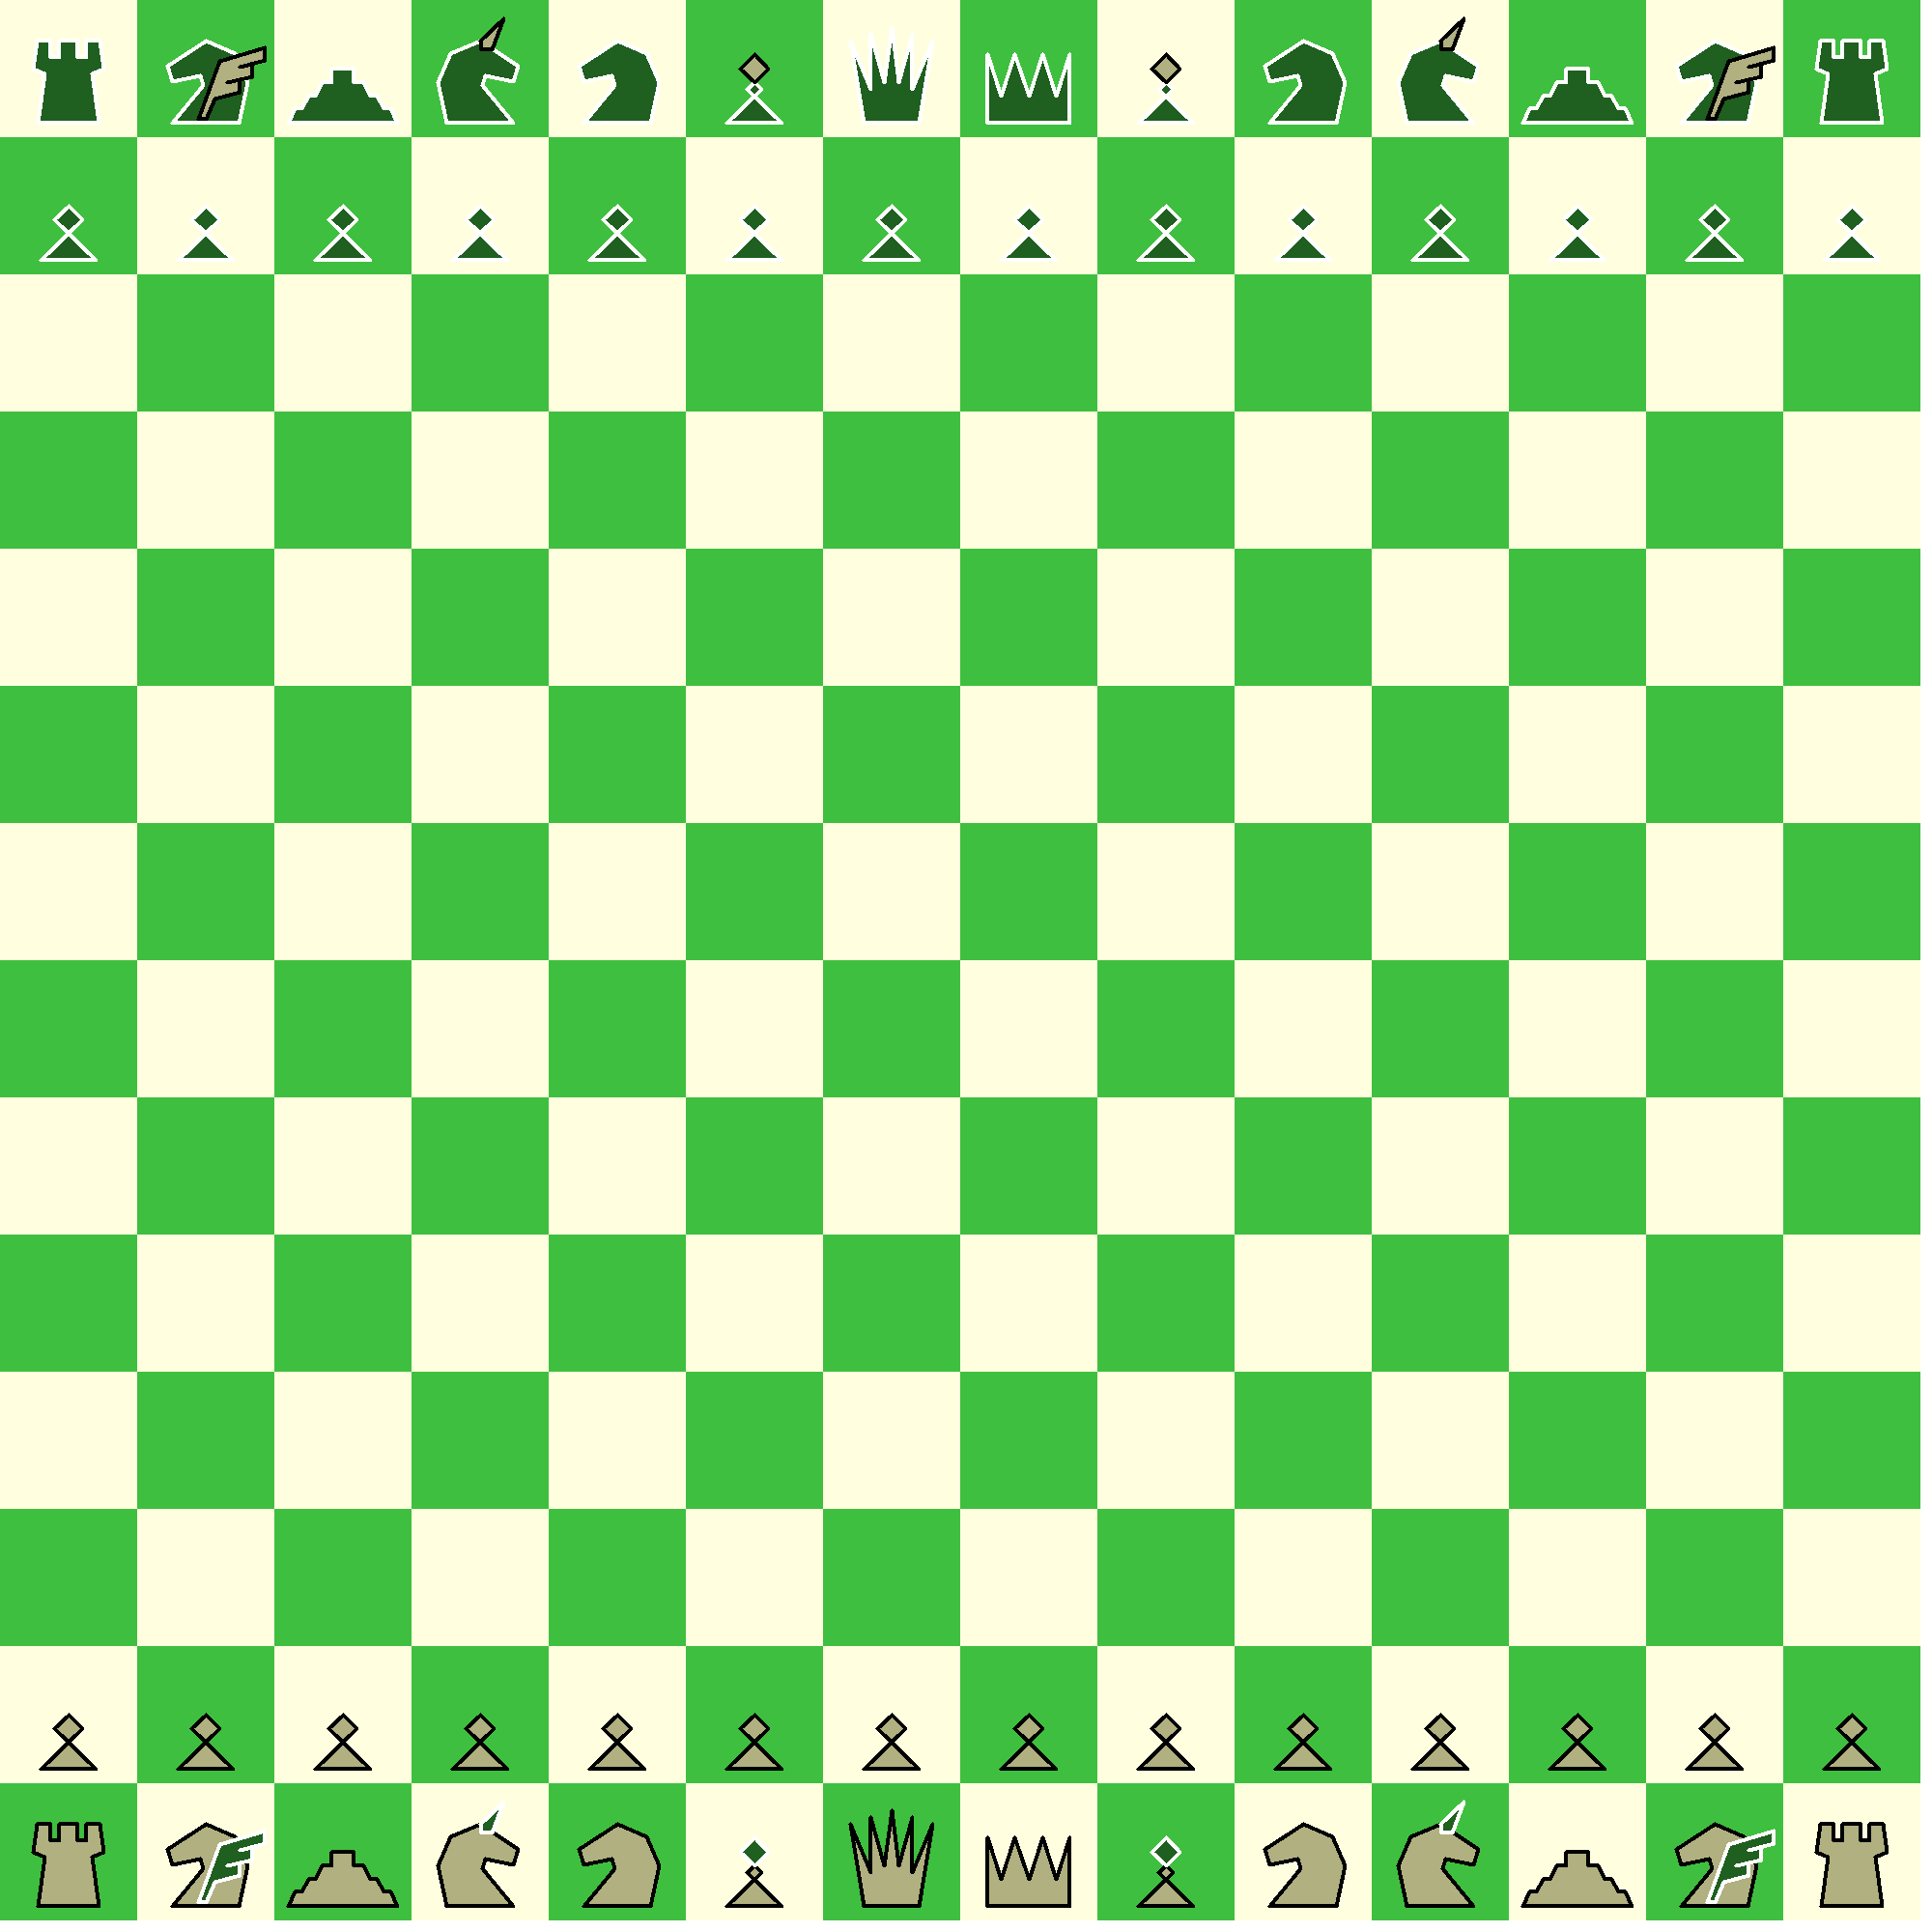
\includegraphics[width=1.0\textwidth, keepaspectratio=true]{boards/08_age_of_aquarius.png}
\caption{Age of Aquarius board}
\label{fig:08_age_of_aquarius}
% \centering
\end{figure}

\clearpage % ..........................................................
% --------------------------------------------- Age of Aquarius chapter
